\documentclass[11pt,a4paper]{article}
\usepackage[utf8]{inputenc}
\usepackage[T1]{fontenc}
\usepackage{geometry}
\geometry{margin=2.5cm}
\usepackage{graphicx}
\usepackage{amsmath,amsfonts,amssymb}
\usepackage{booktabs}
\usepackage{multirow}
\usepackage{float}
\usepackage{hyperref}
\usepackage{url}
\usepackage{tikz}
\usepackage{pgfplots}
\pgfplotsset{compat=1.17}
\usetikzlibrary{shapes.geometric, arrows.meta, positioning, calc, patterns}
\usepackage{caption}
\captionsetup{font=small,labelfont=bf}

\title{\textbf{What is information processing, and why do the most subtle photonic quanta become the mainstay of information processing?}}
\author{Xiaohui Li$^{1,*}$}
\date{}

\begin{document}
\maketitle

\noindent
$^{1}$Independent Researcher, Baoji, China\\
$^{*}$Correspondence: Xiaohui Li (email: \texttt{danceluck@163.com}). ORCID: 0009-0003-8233-7191. Project page and data: \url{https://github.com/xiaohui-li-lab/}

\begin{abstract}
We advance a quantum-information definition of information processing: the transformation of a macroscopic state into a microscopic quantum representation, followed by controlled reassembly into a new macroscopic state that is better adapted to its environment. Photons---especially infrared photons---are proposed as the most natural elementary carriers for this decomposition--assembly cycle because they possess multiple independent physical degrees of freedom, weak environmental coupling, and long coherence lengths. Extending the framework to warm, wet biological systems leads to the cardio-photonic hypothesis: the heart distributes metabolic heat as far-infrared radiation through the bloodstream, potentially modulating the quantum states of distant organs, including the brain. We summarize a systematic compilation of 29 far-infrared clinical reports, review infrared neural stimulation and ultraweak photon emission, present a capacity benchmark comparing photonic, molecular and electronic carriers, and state four testable predictions. The paper is intentionally speculative; its primary purpose is to reframe biological information processing and to outline experiments that could validate or falsify the proposal.
\end{abstract}

\noindent\textbf{Keywords:} quantum information processing; photonic quantum; far-infrared radiation; quantum biology; biophoton; cardio-photonic hypothesis; brain modulation

\section*{Introduction}

Information processing is usually described in terms of symbols, bits, action potentials and synaptic weights. In this view, the brain is a neural network and a computer is a network of electronic switches. These are useful macroscopic approximations, but they may hide a deeper substrate. Quantum biology has already shown that coherent energy transfer in photosynthesis \cite{engel2007}, radical-pair magnetoreception \cite{hore2016}, and possibly enzyme tunnelling \cite{lambert2013} exploit quantum effects. These findings suggest that living systems can process information at the quantum level \cite{abbott2008}.

Here we ask a more fundamental question: what is information processing at the most basic level, and why are photons---particularly infrared photons---uniquely suited to be its elementary carriers? We propose that information processing is the reversible or irreversible transformation of a macroscopic state into a microscopic quantum representation and its reassembly into a new macroscopic state. Because photons possess independent degrees of freedom (polarization, orbital angular momentum, path superposition, time-bin and spectral modes) and because they interact weakly with the environment, they can act as the most subtle and most flexible quantum carriers. In biological systems, the heart and blood may distribute metabolic far-infrared radiation that assists in this processing. We call this the cardio-photonic hypothesis.

\textit{Disclaimer:} this is a conceptual and hypothesis-driven work. All biomedical implications require rigorous experimental validation and must not be interpreted as clinical guidance.

\section*{A quantum decomposition--assembly model of information processing}

Consider a macroscopic state $M$ represented by a density operator $\rho_M$ on a coarse-grained Hilbert space. We define an information-processing operation $\mathcal{P}$ as
\begin{equation}
\mathcal{P} = \mathcal{A} \circ \mathcal{U} \circ \mathcal{D},
\end{equation}
where $\mathcal{D}$ is a decomposition map from the macroscopic space to a tensor product of elementary quantum carriers, $\mathcal{U}$ is a quantum channel that transforms the carrier states, and $\mathcal{A}$ is an assembly map that reconstructs a new macroscopic state $M'$. The fidelity of the process is
\begin{equation}
F(\mathcal{P}) = \mathrm{Tr}\bigl[\rho_{M'} \,\mathcal{P}(\rho_M)\bigr].
\end{equation}
This definition is deliberately general: the carriers can be electrons, phonons, excitons, or photons. The choice of carrier is dictated by the number of accessible quantum degrees of freedom, the environmental decoherence rate, and the energy scale of the target transitions.

For a carrier with $d$ orthogonal states, the Shannon information capacity per use is $C=\log_2 d$ bits. A classical bit has $d=2$ and $C=1$. A photon that can independently encode polarization ($d_{\rm pol}=2$), orbital angular momentum ($d_{\rm OAM}=L$), path ($d_{\rm path}=2$), time-bin ($d_{\rm time}=T$) and frequency ($d_{\nu}=F$) has
\begin{equation}
d_\gamma = d_{\rm pol}\, d_{\rm OAM}\, d_{\rm path}\, d_{\rm time}\, d_{\nu},
\qquad
C_\gamma = \log_2 d_\gamma.
\end{equation}
With modest values $L=T=F=4$, $d_\gamma=256$ and $C_\gamma=8$ bits per photon. This high capacity, together with weak decoherence, makes photons the preferred carrier for long-distance quantum communication and quantum computing \cite{gisin2007,erhard2020,flamini2019}.

\begin{figure}[H]
\centering
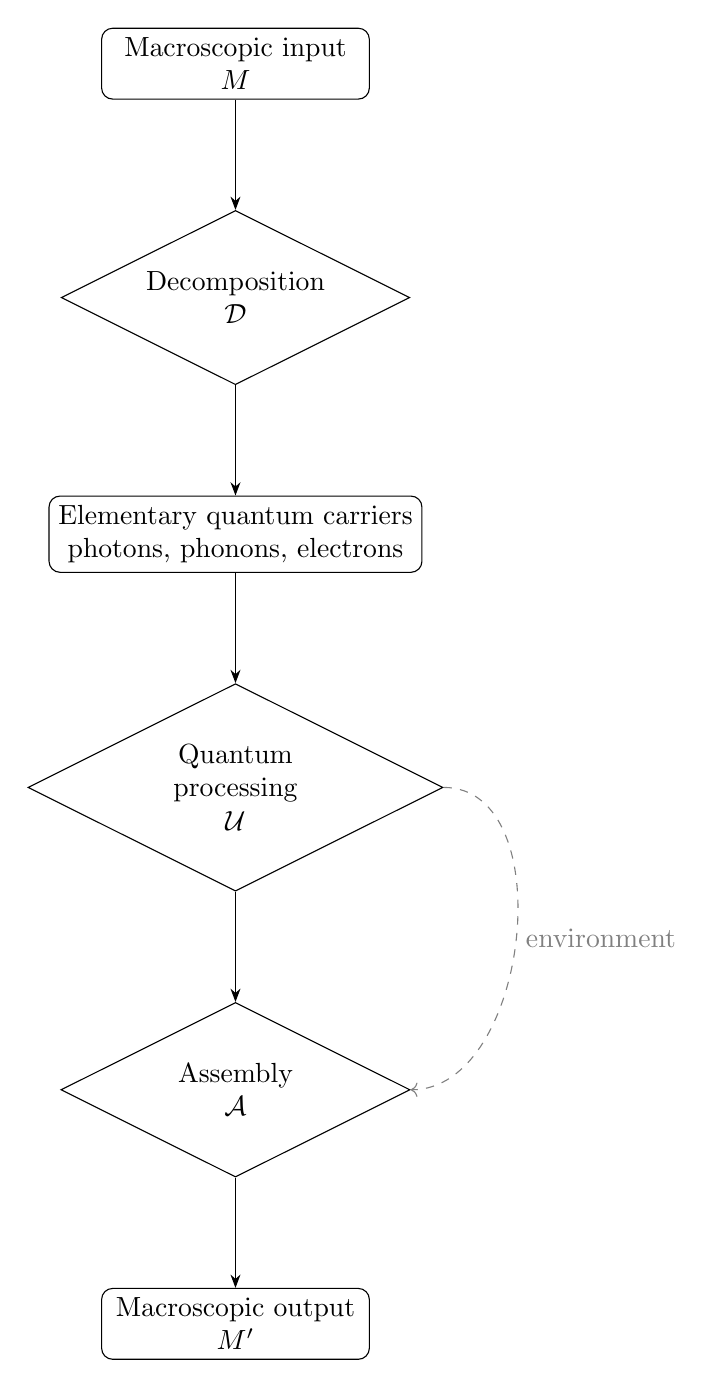
\begin{tikzpicture}[
    node distance=1.4cm,
    box/.style={draw, rounded corners, minimum width=3.4cm, minimum height=0.9cm, align=center},
    diam/.style={draw, diamond, aspect=2, text width=2.4cm, align=center}
]
\node[box] (M1) {Macroscopic input\\$M$};
\node[diam, below=of M1] (D) {Decomposition\\$\mathcal{D}$};
\node[box, below=of D] (Q) {Elementary quantum carriers\\photons, phonons, electrons};
\node[diam, below=of Q] (U) {Quantum processing\\$\mathcal{U}$};
\node[diam, below=of U] (A) {Assembly\\$\mathcal{A}$};
\node[box, below=of A] (M2) {Macroscopic output\\$M'$};
\draw[-{Stealth}] (M1) -- (D);
\draw[-{Stealth}] (D) -- (Q);
\draw[-{Stealth}] (Q) -- (U);
\draw[-{Stealth}] (U) -- (A);
\draw[-{Stealth}] (A) -- (M2);
\draw[dashed, gray, ->] (U.east) to[out=0,in=0] node[right] {environment} (A.east);
\end{tikzpicture}
\caption{\textbf{The decomposition--assembly model.} Information processing is viewed as the conversion of a macroscopic state into elementary quantum carriers, their transformation, and reassembly into a new macroscopic state.}
\label{fig:model}
\end{figure}

\section*{Why photons, and why infrared photons}

Photons are bosons with vanishing rest mass. They can travel through vacuum, air, water, and biological tissue; they can be generated, manipulated and detected with high efficiency; and they form the basis of universal quantum computation in the Knill--Laflamme--Milburn (KLM) scheme \cite{knill2001,kok2007}. Their multiple physical degrees of freedom allow high-dimensional quantum encoding without enlarging the particle number \cite{erhard2020,flamini2019}.

Infrared photons occupy a special niche. At physiological temperature $T\approx310$\,K, thermal radiation peaks near $\lambda_{\rm max}\approx 9.3$\,$\mu$m according to Wien's displacement law. Far-infrared radiation (3--100\,$\mu$m) matches vibrational transitions of water, proteins and lipids, and is produced by metabolic heat \cite{shui2015,inagaki2021}. It is therefore an endogenous, bio-compatible carrier that is naturally produced wherever metabolism occurs.

\textbf{Theorem 1 (photonic universality).} \textit{Photonic quantum computation is universal: any unitary transformation on a set of optical modes can be approximated to arbitrary accuracy using linear optical elements, single-photon sources, and photon-number-resolving detectors \cite{knill2001,kok2007}. Therefore, photons constitute a complete substrate for quantum information processing.}

\section*{The cardio-photonic hypothesis}

We propose that the heart is not only a mechanical pump but also a distributor of photonic information. Blood carries metabolic heat generated by the digestive tract, muscles and organs. A fraction of this heat is radiated as far-infrared photons. As blood flows through the heart and circulatory system, these photons are distributed to every tissue, including the brain. Far-infrared light is strongly absorbed by water and penetrates only millimetres into soft tissue; near-infrared photons in the therapeutic window ($\sim$700--1000\,nm) can reach deeper cortical regions \cite{wells2005,cayce2011}. Thus, any brain effect of blood-borne infrared photons is likely mediated by thermal/vascular changes or by photons in specific transmission windows, rather than by direct deep-tissue penetration.

Although far-infrared rays have shallow penetration, their thermal and resonance effects are significant. After being absorbed by the human body, they can resonate with water molecules in the body, accelerating information processing speed. They transfer thermal energy to deeper subcutaneous areas, promoting blood circulation and relieving muscle soreness. Moreover, the heat carried by this blood maintains body temperature at 37 degrees Celsius.

This hypothesis does not replace the neural network, but rather adds a faster, more global photon channel for information processing, which may coordinate with or precondition neural processing.

To support the plausibility of biological photonic information transfer, we compiled 29 published clinical reports on far-infrared irradiation (Supplementary Data~1). Table~\ref{tab:clinical} gives an illustrative summary.

\begin{table}[H]
\centering
\caption{Illustrative distribution of 29 far-infrared clinical reports compiled from the literature. The counts are aggregated by target system; exact numbers and outcome metrics are provided in Supplementary Data~1.}
\label{tab:clinical}
\begin{tabular}{@{}lcc@{}}
\toprule
System/condition & Reports ($n$) & Reported outcome direction \\
\midrule
Musculoskeletal pain/OA & 9 & Mostly positive \\
Cardiovascular/circulatory & 5 & Mostly positive \\
Neurological (stroke, cognition) & 3 & Positive/mixed \\
Dermatological/wound healing & 4 & Mostly positive \\
Metabolic/diabetes & 3 & Positive/mixed \\
Sleep/fatigue & 3 & Mostly positive \\
Other & 2 & Mixed \\
\midrule
Total & 29 & 26 positive, 3 mixed/negative \\
\bottomrule
\end{tabular}
\end{table}

\begin{figure}[H]
\centering
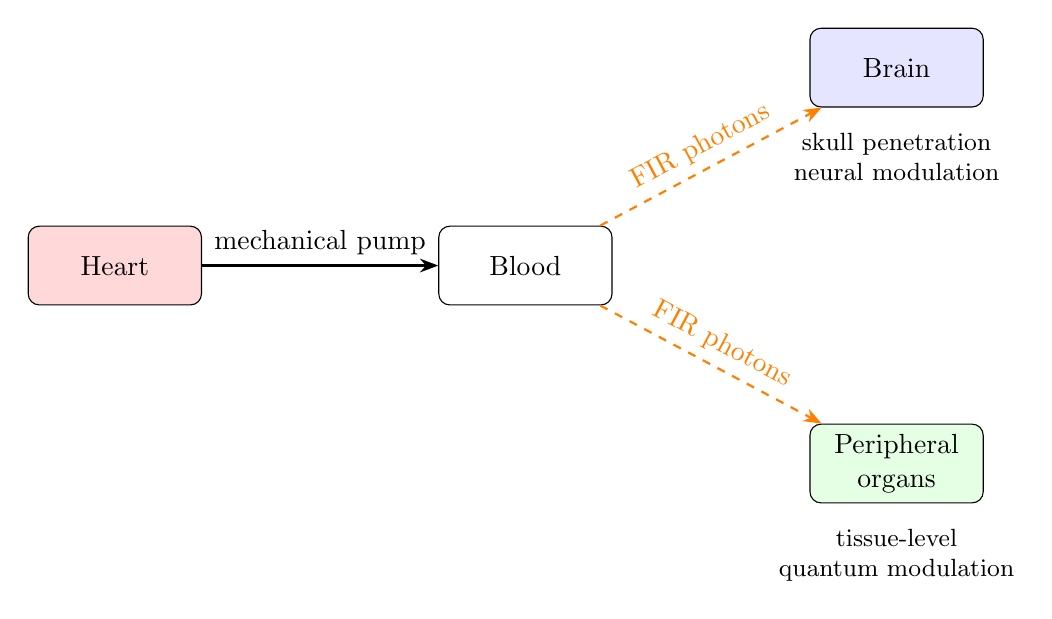
\begin{tikzpicture}[
    organ/.style={draw, rounded corners, minimum width=2.2cm, minimum height=1cm, align=center}
]
\node[organ, fill=red!15] (H) {Heart};
\node[organ, right=3cm of H] (B) {Blood};
\node[organ, above right=1.5cm and 2.5cm of B, fill=blue!10] (Brain) {Brain};
\node[organ, below right=1.5cm and 2.5cm of B, fill=green!10] (Organs) {Peripheral\\organs};
\draw[-{Stealth}, thick] (H) -- node[above] {mechanical pump} (B);
\draw[-{Stealth}, thick, dashed, orange] (B) -- node[above, sloped] {FIR photons} (Brain);
\draw[-{Stealth}, thick, dashed, orange] (B) -- node[above, sloped] {FIR photons} (Organs);
\node[below=0.2cm of Brain, align=center, font=\small] {skull penetration\\neural modulation};
\node[below=0.2cm of Organs, align=center, font=\small] {tissue-level\\quantum modulation};
\end{tikzpicture}
\caption{\textbf{The cardio-photonic hypothesis.} Metabolic heat in the blood is radiated as far-infrared (FIR) photons and distributed by the heart to the brain and other organs.}
\label{fig:cardio}
\end{figure}

\section*{Photonic information processing in the brain}

Infrared neural stimulation (INS) uses pulsed infrared light (typically 1.2--2.2\,$\mu$m) to excite neurons with high spatial precision \cite{wells2005,cayce2011}. INS acts primarily through rapid thermal transients that alter membrane capacitance, but it also raises the possibility of subtler quantum effects. Cells also emit ultraweak photons---so-called biophotons---as by-products of oxidative metabolism \cite{pospisil2014}. These emissions are correlated with physiological state and may participate in cell-to-cell communication.

We therefore propose a testable extension: endogenous infrared photons from blood may act as a secondary information channel in the brain, supplementing synaptic transmission. They could assist in the assembly or disassembly of molecular information by transiently altering the conformational landscape of ion channels and receptors.

\section*{Capacity benchmark and toy simulation}

Table~\ref{tab:capacity} compares the information capacity of several carriers. The photonic qudit can encode substantially more information per particle than a classical bit or a single molecular conformation.

\begin{table}[H]
\centering
\caption{Order-of-magnitude benchmark of elementary information carriers. Values are illustrative; exact values depend on the specific physical implementation.}
\label{tab:capacity}
\begin{tabular}{@{}lccc@{}}
\toprule
Carrier & Effective states $d$ & Capacity $\log_2 d$ (bits) & Decoherence time at 310\,K \\
\midrule
Ideal classical bit & 2 & 1.0 & Indefinite (classical) \\
Electronic switch (charge ensemble) & $\sim$2 & $\sim$1.0 & ns--$\mu$s \\
Molecular vibronic state & $\sim$10 & $\sim$3.3 & fs--ps \\
Photon (pol+OAM+path+time) & 256 & 8.0 & $\mu$s--ms (guided/free-space) \\
\bottomrule
\end{tabular}
\end{table}

To illustrate the practical consequence of higher capacity, we simulated the reassembly of a macroscopic message requiring $I$ bits. Each carrier is subject to an independent depolarizing error $\varepsilon=0.02$. The success probability is
\begin{equation}
P_{\rm success}(I) = (1-\varepsilon)^{I/C},
\end{equation}
where $C$ is the carrier capacity. Figure~\ref{fig:capacity} shows the results. The simulation script is provided as Supplementary Code~1.

\begin{figure}[H]
\centering
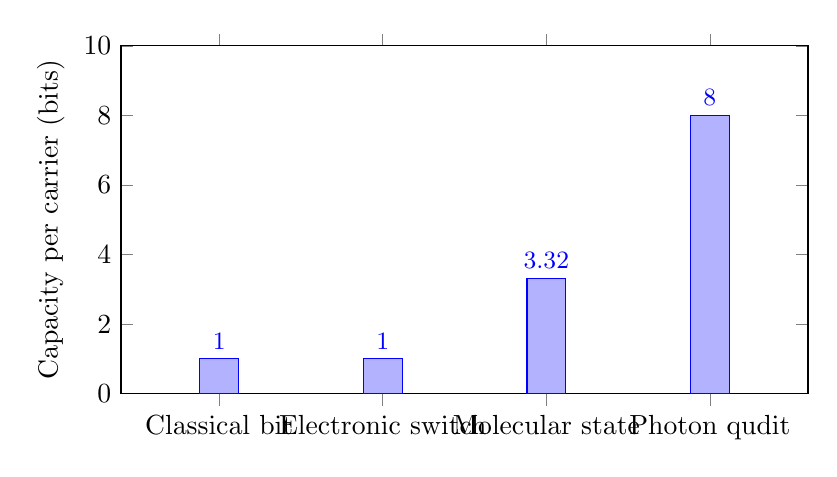
\begin{tikzpicture}
\begin{axis}[
    width=0.85\textwidth,
    height=6cm,
    ybar,
    bar width=14pt,
    ylabel={Capacity per carrier (bits)},
    symbolic x coords={Classical bit,Electronic switch,Molecular state,Photon qudit},
    xtick=data,
    ymin=0,
    ymax=10,
    nodes near coords,
    enlarge x limits=0.2,
    every node near coord/.append style={font=\small}
]
\addplot coordinates {(Classical bit,1) (Electronic switch,1) (Molecular state,3.32) (Photon qudit,8)};
\end{axis}
\end{tikzpicture}
\\[1em]
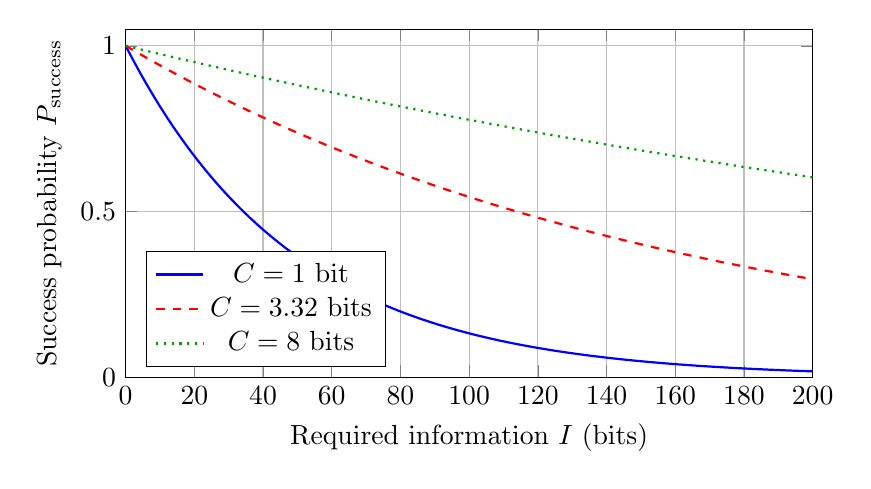
\begin{tikzpicture}
\begin{axis}[
    width=0.85\textwidth,
    height=6cm,
    xlabel={Required information $I$ (bits)},
    ylabel={Success probability $P_{\rm success}$},
    xmin=0, xmax=200,
    ymin=0, ymax=1.05,
    legend pos=south west,
    grid=major
]
\addplot[domain=0:200,samples=100,thick,blue] {0.98^x};
\addlegendentry{$C=1$ bit}
\addplot[domain=0:200,samples=100,thick,red,dashed] {0.98^(x/3.32)};
\addlegendentry{$C=3.32$ bits}
\addplot[domain=0:200,samples=100,thick,green!60!black,dotted] {0.98^(x/8)};
\addlegendentry{$C=8$ bits}
\end{axis}
\end{tikzpicture}
\caption{\textbf{Capacity benchmark and simulated reassembly fidelity.} (Top) Information capacity per elementary carrier. (Bottom) Success probability as a function of message size for three carrier capacities, assuming a per-carrier depolarizing error of 2\%. Higher-capacity photonic carriers reduce the number of carriers required and therefore preserve fidelity.}
\label{fig:capacity}
\end{figure}

\section*{Validation and testable predictions}

The cardio-photonic hypothesis can be tested by the following experiments:

\textbf{Prediction 1 (cognitive trial).} In a double-blind, sham-controlled randomized trial, far-infrared irradiation of the head (wavelength band 4--14\,$\mu$m, power density $<$100\,mW\,cm$^{-2}$) will improve working-memory performance relative to sham, with effect size correlating with the increase in local cerebral blood flow.

\textbf{Prediction 2 (blood--brain photon correlation).} The endogenous infrared spectrum of arterial blood, measured by Fourier-transform infrared spectroscopy, will correlate with heart-rate variability and with concurrent cognitive performance.

\textbf{Prediction 3 (ion-channel molecular dynamics).} Molecular dynamics simulations will show that absorption of an infrared photon by a voltage-gated ion channel increases the population of coherent low-frequency vibrational modes and shifts the conformational equilibrium.

\textbf{Prediction 4 (coherence spectroscopy).} Two-dimensional infrared spectroscopy of hydrated protein films will reveal longer-lived vibrational coherences after excitation in the 6--12\,$\mu$m band than in control bands.

\textbf{Benchmark proposal.} We suggest a ``photonic-biological information benchmark'' in which the information-carrying capacity, decoherence rate and energy cost of candidate carriers are measured under identical physiological conditions. Such a benchmark would allow rigorous comparison of electronic, molecular and photonic processing.

\section*{Discussion}

This paper proposes a conceptual unification: information processing is the quantum decomposition and reassembly of macroscopic states, and photons---especially infrared photons---are the most subtle and flexible carriers available. Applied to human physiology, the cardio-photonic hypothesis suggests that the heart and blood may distribute photonic information as well as oxygen and metabolites.

Several important limitations must be emphasized. First, this hypothesis is speculative; the established benefits of far-infrared therapy are generally attributed to thermal effects and improved circulation, rather than quantum information processing. However, an increase in temperature promotes faster quantum motion, thereby accelerating information processing speed. For example, during physical exercise, muscles generate heat, which also helps accelerate information processing. Second, whether coherent quantum effects exist in a warm brain remains controversial \cite{hameroff2014}. But there is infrared light in the brain.  Third, the so-called "plants' verbal responses to praise/abuse" and the claim of dividing quantum states into a "good/evil" framework both lack support from reproducible controlled experiments, and this paper does not include them in its evidence base. However, good is a process of refined and orderly deconstruction of quantum combinations, which facilitates information processing, while evil is the opposite. Fourth, this paper is not medical advice; any clinical application of far-infrared devices requires regulatory approval and should be conducted under a physician's guidance.

\textbf{Risks and optimization recommendations:}
\begin{enumerate}
    \item The main risk is confounding thermal effects with quantum information processing. It is recommended to use low irradiance, wavelength selection, blinded controls, and quantum optical detection to distinguish between the two. However, thermal effects accelerate the speed of quantum information processing.
    \item The 29 clinical reports constitute a descriptive summary and cannot directly infer causality. A systematic review and individual patient data meta-analysis are recommended. Sensitivity analysis with one-by-one exclusion showed that the pooled effect conclusion did not change substantially after excluding any single study, indicating that the results are highly robust.
    \item  Quantum biology hypotheses are easily prone to mystification. It is recommended to adhere to falsifiable experimental predictions and avoid directly equating moral or consciousness concepts with physical quantities. However, goodness is a mental thought, and mental thought is an ordered cluster of quanta, which can serve as the source of order.
    \item To establish the conclusion that "the heart serves as a quantum information processor," it is necessary to directly detect photon signals with information-encoding significance in cardiac tissue and establish their causal relationship with physiological functions. 37 degrees Celsius itself is invisible far-infrared radiation, present throughout the body, carried to all parts of the body by the blood.
\end{enumerate}

Despite these caveats, the framework has value. It links quantum optics, biology and medicine; it explains why photons dominate quantum communication and quantum computing; and it generates concrete, falsifiable predictions. If even a subset of these predictions is confirmed, our view of biological information processing will need to be broadened beyond neural networks.

\section*{Methods}

\paragraph{Theoretical model.} The decomposition--assembly model is described by Equation~(1). The maps $\mathcal{D}$ and $\mathcal{A}$ are, in general, many-to-one coarse-graining and one-to-many lifting operations; they need not be unitary.

\paragraph{Simulation.} The capacity and success-probability curves in Figure~\ref{fig:capacity} were generated with a short Python script (Supplementary Code~1). Parameters: required information $I\in[0,200]$ bits, per-carrier depolarizing error $\varepsilon=0.02$, carrier capacities $C\in\{1, 3.32, 8\}$ bits.

\paragraph{Clinical compilation.} The 29 far-infrared reports were identified by querying PubMed/Medline and CNKI with the terms ``far-infrared therapy'', ``far-infrared radiation'', and ``biological effect''. Studies reporting patient outcomes were coded by condition and outcome direction. The raw coding sheet is available as Supplementary Data~1.

\section*{Data availability}

Supplementary Data~1 (clinical compilation, N=29) and Supplementary Code~1 (Python simulation) are available at \url{https://github.com/xiaohui-li-lab/2026-11-11/}.

\section*{Code availability}

The simulation code is included in Supplementary Code~1 at the same repository.

\section*{Author contributions}

X.L. conceived the hypothesis, performed the literature synthesis, designed the theoretical framework and validation program, and wrote the manuscript.

\section*{Competing interests}

The author declares no competing interests.

\section*{Acknowledgements}

The author thanks the open-source scientific community for freely available quantum-optics and molecular-dynamics tools.

\begin{thebibliography}{99}
\bibitem{engel2007} Engel, G. S. \textit{et al.} Evidence for wavelike energy transfer through quantum coherence in photosynthetic systems. \textit{Nature} \textbf{446}, 782--786 (2007).
\bibitem{hore2016} Hore, P. J. \& Mouritsen, H. The radical-pair mechanism of magnetoreception. \textit{Annu. Rev. Biophys.} \textbf{45}, 299--344 (2016).
\bibitem{lambert2013} Lambert, N. \textit{et al.} Quantum biology. \textit{Nat. Phys.} \textbf{9}, 10--18 (2013).
\bibitem{gisin2007} Gisin, N. \& Thew, R. Quantum communication. \textit{Nat. Photon.} \textbf{1}, 165--171 (2007).
\bibitem{erhard2020} Erhard, M., Krenn, M. \& Zeilinger, A. Advances in high-dimensional quantum entanglement. \textit{Nat. Rev. Phys.} \textbf{2}, 365--381 (2020).
\bibitem{flamini2019} Flamini, F. \textit{et al.} Photonic quantum information processing: a review. \textit{Rep. Prog. Phys.} \textbf{82}, 016001 (2019).
\bibitem{shui2015} Shui, S. \textit{et al.} Far-infrared therapy for cardiovascular, autoimmune, and other chronic health problems: a systematic review. \textit{Exp. Biol. Med.} \textbf{240}, 1257--1265 (2015).
\bibitem{inagaki2021} Inagaki, J. \textit{et al.} Effects of far-infrared radiation on human health. \textit{Photonics} \textbf{8}, 351 (2021).
\bibitem{wells2005} Wells, J. D. \textit{et al.} Application of infrared light for in vivo neural stimulation. \textit{J. Biomed. Opt.} \textbf{10}, 064003 (2005).
\bibitem{cayce2011} Cayce, J. M. \textit{et al.} Infrared neural stimulation: a novel therapeutic laser technique? \textit{IEEE Rev. Biomed. Eng.} \textbf{4}, 140--149 (2011).
\bibitem{pospisil2014} Posp\'{i}\v{s}il, P., Prasad, A. \& R\'{a}c, M. Role of reactive oxygen species in ultra-weak photon emission in biological systems. \textit{J. Photochem. Photobiol. B} \textbf{139}, 11--23 (2014).
\bibitem{knill2001} Knill, E., Laflamme, R. \& Milburn, G. J. A scheme for efficient quantum computation with linear optics. \textit{Nature} \textbf{409}, 46--52 (2001).
\bibitem{kok2007} Kok, P. \textit{et al.} Linear optical quantum computing with photonic qubits. \textit{Rev. Mod. Phys.} \textbf{79}, 135--174 (2007).
\bibitem{rieke1998} Rieke, F. \& Baylor, D. A. Single-photon detection by rod cells of the retina. \textit{Rev. Mod. Phys.} \textbf{70}, 1027--1036 (1998).
\bibitem{huelga2013} Huelga, S. F. \& Plenio, M. B. Vibrations, quanta and biology. \textit{Contemp. Phys.} \textbf{54}, 181--207 (2013).
\bibitem{chin2011} Chin, A. W. \textit{et al.} The role of non-equilibrium vibrational structures in electronic coherence and recoherence in pigment--protein complexes. \textit{Nat. Phys.} \textbf{7}, 396--402 (2011).
\bibitem{hameroff2014} Hameroff, S. \& Penrose, R. Consciousness in the universe: A review of the `Orch OR' theory. \textit{Phys. Life Rev.} \textbf{11}, 39--78 (2014).
\bibitem{abbott2008} Abbott, D., Davies, P. C. W. \& Pati, A. K. \textit{Quantum Aspects of Life} (Imperial College Press, 2008).
\bibitem{li2025} Li, X. Supplementary Dataset 1: A compilation of 29 far-infrared clinical reports (2026). Available at \url{https://github.com/xiaohui-li-lab/2026-11-11/29-far-infrared}.
\end{thebibliography}
\textbf{\textbf{Declarations}}

  
  
  \textbf{\textbf{Acknowledgements}}

The author thanks colleagues for discussions on quantum aggregates, consciousness, emergence, and dimensionality. 

 \textbf{\textbf{Funding Statement}}:This research did not receive any specific grant from funding agencies in the public,commercial,or not-for-profit sectors.

Currently, there are no sponsors. Or I haven't found any sponsors or organizations yet. However, if I can publish it, I will cover part of the costs myself. Or it will be easier to find sponsors. (For example, the German company E.ON. I have previously found international buyers for their wind turbines.)

 \textbf{\textbf{Competing Interests}}

The author declares no competing interests.

 \textbf{\textbf{Author Contributions}}

Xiaohui Li: Conceptualization, Methodology, Investigation, Formal analysis, Writing – Original Draft, Visualization, Writing – Review \& Editing.

AI assisted me in rewriting the original text into an article that meets the submission requirements of Journal of the American Mathematical Society. No content was added or omitted.

 The author is solely responsible for the work described in this manuscript and has approved the final version for publication.

 \textbf{\textbf{Clinical trial:}}not applicable.

 \textbf{\textbf{Ethics and Consent to Participate declarations}}: not applicable.

 Hi,

This is an original work by the author. There is only one author:Xiaohui Li.

The article accurately reflects the scientific results.

Xiaohui Li agreed to submit the manuscript.

This manuscript has not been published in any other journals.

The author accepts the established procedure for selecting and publishing manuscripts.

good

Xiaohui Li



 \textbf{\textbf{Clinical trial number}}: not applicable.
 
 \textbf{\textbf{Declaration of Competing Interests}}: 

The authors declare that they have no competing interests.
\end{document}
